\RequirePackage{snapshot}
\documentclass [10pt, fancyhdr, twoside] {article}
\usepackage{float, graphicx, caption, amssymb, natbib}
\usepackage[usenames,dvipsnames]{color}
\usepackage{tabulary}
\usepackage [left=2.5cm, top=2.5cm, bottom=2.5cm, right=3cm] {geometry}  %% see geometry.pdf on how to lay out the page. There's lots.
\geometry{a4paper} %% or letter or a5paper or ... etc
\usepackage{fancyhdr}
\usepackage{xcolor}
\usepackage[scaled]{helvet}
\usepackage{tcolorbox}
\usepackage{enumitem}
\usepackage{bbding}
\usepackage{tikz}

\renewcommand*\familydefault{\sfdefault} %% Only if the base font of the document is to be sans serif

\usepackage[left]{lineno}
\usepackage[yyyymmdd,hhmmss]{datetime}

\renewcommand{\linenumberfont}{\normalfont\tiny\color{gray}}


\pagestyle{fancy}

\fancyhf{}

%\fancyhead{}
%\fancyfoot{}

%\fancyhf{}
%\fancyhead[RO,LE]{Heading}
%\fancyfoot[RO,LE]{}
\fancyfoot[C]{\thepage}
%\fancyfoot[RE, LO]{}

%\sectionfont{\centering}
%\subsectionfont{\centering}
\setcounter{secnumdepth}{0}

\usepackage{blindtext}

\newcounter {note}
\stepcounter{note}

\renewcommand{\abstractname}{Abstract Name}

\newcommand {\Note} [1] {
    \marginpar {
        \tiny {
            {\color{gray}{\thenote  \  #1}}
            }
        }
    \stepcounter {note}
}

\newcommand {\MNote} [1] {
    \marginpar {
        \tiny {
            {\color{gray}{#1 }}
            }
        }
}

\begin{document}

\title{Analýza \textsc{Cash Flow} \\
  \large Metoda pro hodnotový management \\
}


\author{
  Ing. Karel Hubálek, CSc.
  \and
  RNDr. Edvard Špaček
}
\date{}


\maketitle

\newcommand\HRule{\rule{\textwidth}{1pt}}

\begin{center}

\HRule \\[0.4cm]
{ \huge \bfseries \textsc{\LARGE Vesna 1} / \textsc{\LARGE Vesna 2}  }\\[0.4cm]

\HRule \\[2cm]

\end{center}


\section{Význam metody}

Metoda \textsc{Vesna} transformuje ekenomické parametry výrobního programu složeného z jednotlivých akcí do finančního toku podniku. Jediná tohoto druhu originální metoda Vám zaplní výrboní program přednostně efektivními akcemi (výrobky, službami).

Každý podnikatel může z výsledku analýzy podle metody \textsc{Vesna} získat informaci, jak se parametry akce jím navrhované projeví na hospodářských výsledcích firmy. Analýza podnikatelských záměrů metodou \textbf{finančních toků} vede k docílení maximální efektivnosti a tím zakládá budoucí \textbf{prosperitu firmy}.

Pro management podniku poskytuje metod \textsc{Vesna} výsledky analýzy finančního toku  za celý výrobní program, složený z jednotlivých akcí. Z takového rozboru se dají odvodit především budoucí čisté získy hospodářských jednotek odvozené z konkrétní volby výrobkové strategie v rozvojovém záměru. Očekávané budoucí zisky jsou nejspolehlivějším východiskem pro stanovování tržní hodnoty podniků v procesu jejich privatizace. Metoda poskytuje též informace pro posuzování efektivnosti investinčních akcí. Využití metody \textsc{Vesna} tak dokládá \textbf{privatizační projekty} a \textbf{investiční záměry}.

\textbf{Znalost docílitelné výše celkového zisku pro zvolený výrobní program umožňuje podnikům zařadit do něho i relativně ztrátové akce a udžet si pozice na trhu i zaměstnanost}.

\section{Co metoda přináší}

Ve výpočtu se získají jak pro jednotlivé akce, tak pro celý podnik (i pro dílčí program) ukazatele, které jsou ve světové ekonomice všeobecně uplatňovány, zejména:

\begin{itemize}[label=\NibRight]
\item Současná čistá hodnota efektu (NPV) a její závislost na procentu diskontu, Vnitřní výnosové procento (IRR) vložených investic.
\item Rentabilita výrobních fondů, Doba úhrady investic
\item Minimální počet vyrobených k úhradě investic (bod zvratu)
\end{itemize}

\subsection{Další přístupy uplatněné v metodě \textsc{Vesna}}

\begin{itemize}
\item Analyzují se nejen \textbf{jednotlivé akce} (nová výroba, technologie, služby), ale i jejich \textbf{souhrnné hodnocení} pro celý výrobní program podniku.
\item V souladu s tržními principy je pro jednotlivé akce sledováno respektování zájmů v \textbf{uživatelské oblasti}, tj. nákladovost a efekty v provozu výrobků, podklady pro marketing a zajištění prodejnosti, je doporučena optimálni cena a další.
\item Souhrnné hodnocení umožňuje vedle analýzy finančního toku podniku \textbf{uspořádání akcí} podle efektivnosti a návaznosti na optimální výběr a zaplňování kapacit.
\end{itemize}

\subsection{Postup výpočtu}

\begin{enumerate}
\item Uživatel vyplní při hodnocení jednotlivých akcí tabulku \textsc{Podkladové údaje} akce pro aplikaci metody \textsc{Vesna} 92 (tab. 1).

Počítač vypíše tabulku \textsc{Výsledky} (tab. 2). Podává přehled o výsledných parametrech akce včetně návrhu její informativní ceny pro výrobek, službu a pod. Dalšímy výstupními sestavami jsou:

\begin{itemize}
\item diagram \textsc{Průběh efektů u výrobce} (obr. 1)
\item diagram \textsc{Závislost efektu na \% diskontu}
\item diagram \textsc{Průběh efektu u uživatele}
\item diagram \textsc{Model užitnosti a rentability} (obr. 2)
\item tabulka \textsc{Podkladové údaje~–~opis} (kontrola vstupů)
\item tabulka \textsc{Užitky, náklady} (rozpis ročních složek)
\item tabulka \textsc{Efekty} (přehled roční a kumulované tvorby)
\end{itemize}

\item Pro \textbf{souhrnné hodnocení} akcí do analýzy finančního toku podniku se vyplní podkladová tabulka \textsc{Výběrový blok} s podmínkami pro zařazení akcí archivovaných z předchozích výpočtů do zvoleného výběru, a zadají limitní kapacity v letech propočtové periody.

Automaticky je vypracována sumarizace jednotlivých akcí po rocích ve variantě \textbf{nekorigované}, tj. pro původní záměr a korigované, v níž se navrhne dle omezené kapacity jen optimální výrobní program. Je nabídnuta řada tabulek a diagramů s analýzou finančního toku podniku. Z tabulek je to např. hlavní sestava: \textsc{Svodné výsledky nekorigované} (tab. 3), z grafů jsou uvedeny
diagram \textsc{Finanční tok podniku~–~nekorigováno} (obr. 3).
diagram \textsc{Zaplnění kapacity podniku~–~korigováno} (obr. 4).

\end{enumerate}

\begin{tcolorbox}

\textbf{Pouze na důsledně efektivních plánech stojí efektivní podnikání!}
\end{tcolorbox}

\newpage

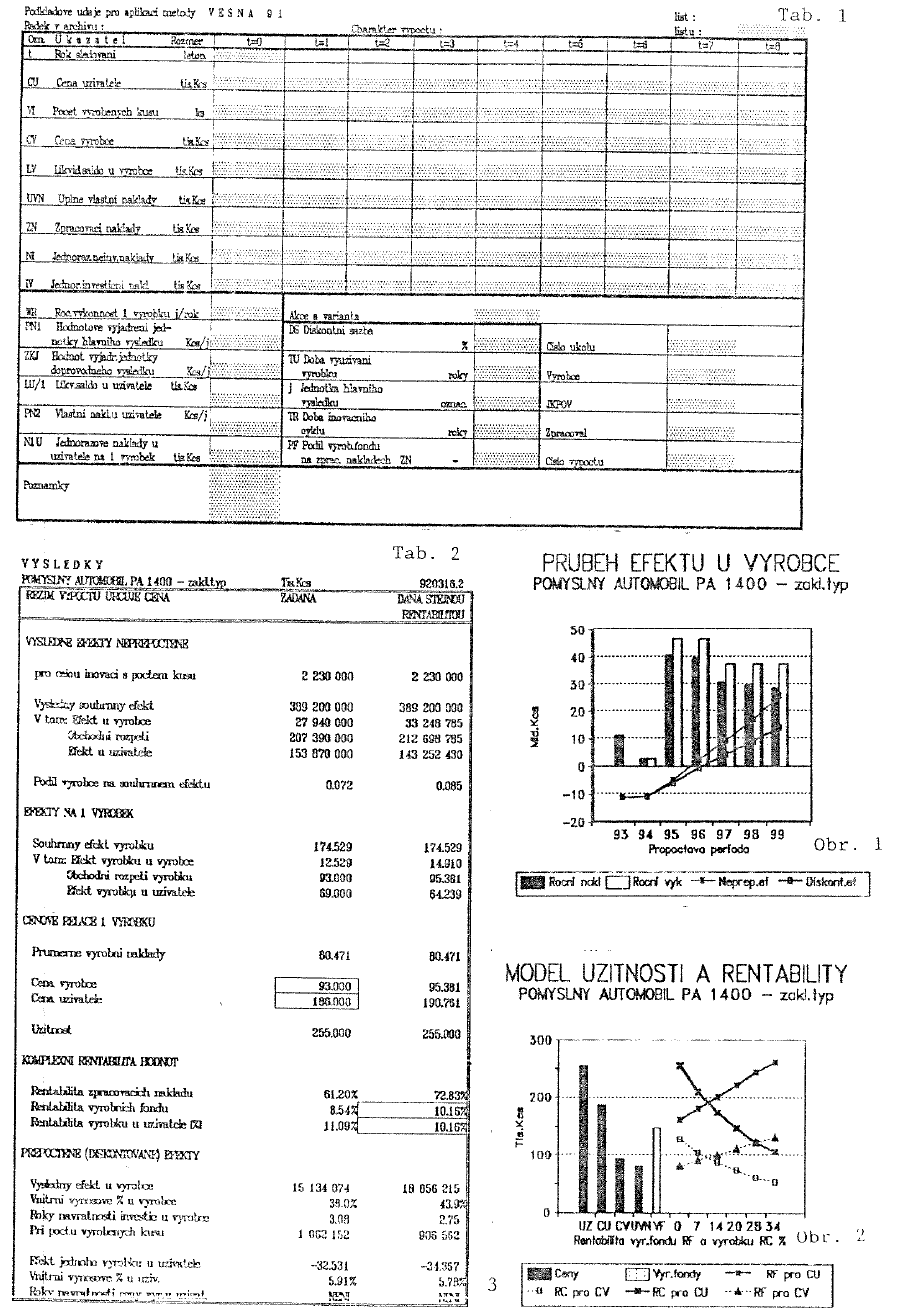
\includegraphics[width=\textwidth,height=\textheight,keepaspectratio]{./vesna-obr1.png}

\newpage

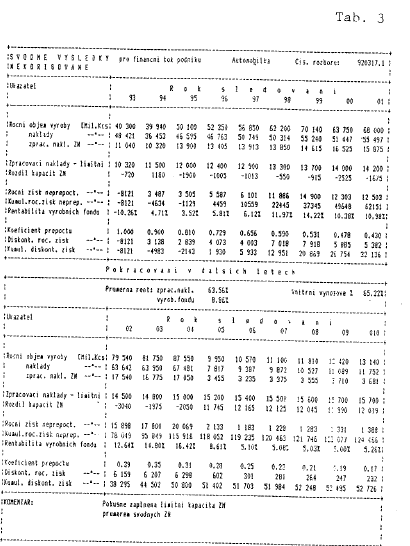
\includegraphics[width=\textwidth,height=\textheight,keepaspectratio]{./vesna-obr2.png}

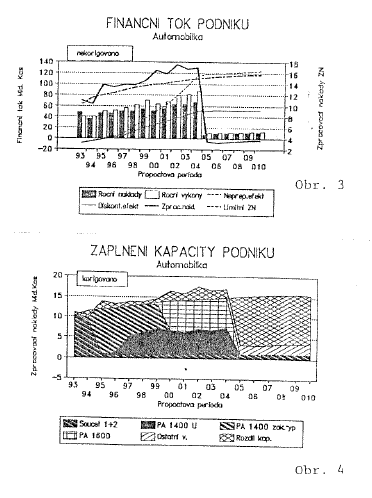
\includegraphics[width=\textwidth,height=\textheight,keepaspectratio]{./vesna-obr3.png}


\end{document}
